
\subsubsection{Project Description}

Teleoperation is a topic of great interest for our research group.
In this project we plan on finding ways to enable the user to operate a remote robot in a intuitive and effective way.
In particular, we would like to investigate ways of simultaneously transmit to the user information on the remote environment (i.e. the forces that the robot is experiencing), as well as guidance towards a desired objective.

The main goal of teleoperation is to provide the user with an immersive feeling of telepresence, i.e. to make the user experience as if he was in the remote environment.
There are however a number of challenges both in the way that the user handles the master device, how it moves the slave robot and how he perceives the remote forces.
In addition, providing cues for guidance as well brings about a number of added difficulties which should be investigated by the student.

\subsubsection{Task Overview}

The task consists of using a telemanipulation system to carry out pick and place tasks. 
The student should investigate how to combine haptic feedback that provides the user with information on the forces on the remote environment and also to be guided towards a good location for grasping that is calculated autonomously.



\begin{figure}[htb!]
	\centering
	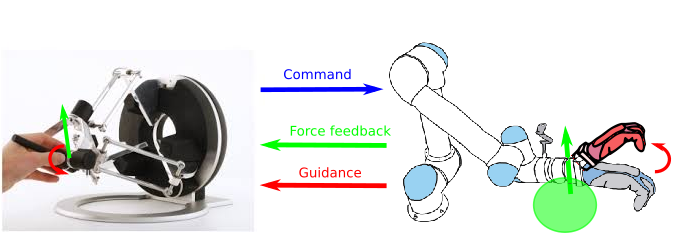
\includegraphics[width=12cm]{teleop}
	\caption{Telemanipulation system with guidance and haptic feedback}
\end{figure}


\subsubsection{Timeline}
\paragraph{Months 1-2}
The student should dedicate the first two months of his project to getting familiar with the hardware and software architecture.
Tutorials and online courses in C++, Python, and ROS (Robot Operating System) programming should be followed, while also learning how to interface with the haptic device.
\paragraph{Months 3-4}
The student should have developed and implemented a number of different strategies for controlling a remote robot and feeding the information back to the user.
\paragraph{Months 5-6}
User studies should be carried out to determine the best strategy for commanding the robot and conveying the relevant information, in view of preparing a scientific article.

\subsubsection{Required Skills}
The successful completion of this project requires that the student possesses or can easily acquire the following skills: 
%\subsection{Technical Skills}
\paragraph{Programming} A significant part of the work will be the development of algorithms and control laws to be executed by the robot. Prototyping is usually done in MATLAB and then implemented in the C++ or Python programming languages.
\paragraph{Linear Algebra} Knowledge of Linear Algebra is essential for developing robot motion control algorithms, particularly  transformations, Jacobian matrices, and matrix operations.
\paragraph{Teleoperation}
Concepts of teleoperation and haptic feedback should be understood.
Passivity theory, kinematic mapping, cutaneous and kinaesthetic feedback, as well as shared control strategies should be studied.

\subsubsection{Outcomes}
The student will become proficient in robot control and teleoperation.
He will also learn how to carry out user studies.
Furthermore, he will have the experience of working in a research environment, obtaining experimental skills, the ability to work independently and in a group. He will also learn how to do data analysis, scientific writing, user studies and programming.
\subsubsection{Suggested Readings}
\begin{itemize}
	\item	\bibentry{pozzi2018closure}
	\item  \bibentry{bimbo2017teleoperation}
	\item \bibentry{chinello2018design}
	\item \bibentry{moreno2018transparency}
\end{itemize}

